\chapter{Robustness of fingerprinting techniques against attacks}\label{sec:Robustness}

\section{Experimental setup}
\subsection{Robustness measures}
Fingerprinting schemes should be robust against different attempts to prevent the correct detection of the fingerprint.
Modifying, deleting and adding the values to the fingerprinted data, that can be both benign updates and malicious attacks, can modify or erase the fingerprint. 
A robust fingerprinting scheme should make it hard for the attacker to erase the fingerprint, to modify it in the way that an innocent buyer is implicated as a traitor, or to modify unmarked data such that a valid fingerprint is detected.

In further sections we analyse robustness fingerprinting schemes against different attacks using robustness measures proposed in \cite{li2005fingerprinting}:
\begin{itemize}
  \item \textbf{Misdiagnosis false hit} $(fh^D)$: The probability of detecting a valid fingerprint from data that has not been fingerprinted.
  \item \textbf{Misattribution false hit} $(fh^A)$: The probability of detection an incorrect but valid fingerprint from fingerprinted data.
  \item \textbf{False negative} $(fn)$: The probability of detecting no valid fingerprint from fingerprinted data.
  \item \textbf{False miss} $(fm)$: The probability of failing to detect an embedded fingerprint correctly. False miss rate is the sum of the false negative and misattribution false hit rates, i.e. $fm=fh^A+ fn$.
\end{itemize}

\subsection{Datasets}\label{datasets}
We use three different datasets for the experiments on fingerprint robustness and quality effects on fingerprinted datasets in the following sections obtained from the UCI Machine Learning repository \cite{Dua:2019}:
\begin{itemize}
    \item Forest Covertype dataset\footnote{\url{https://archive.ics.uci.edu/ml/datasets/covertype}}
    \item German Credit Data\footnote{\url{https://archive.ics.uci.edu/ml/datasets/statlog+(german+credit+data)}}
    \item Adult dataset (train data)\footnote{\url{https://archive.ics.uci.edu/ml/datasets/adult}}
\end{itemize}
\paragraph{Forest Cover Type}
The dataset contains measurements related to the forest cover originally obtained from US Geological Survey (USGS) and US Forest Service (USFS) data.
This dataset is chosen due to its desired properties of containing multiple integer-valued attributes, because of its size and because its intended purpose is the classification problem with target \textit{Cover\_Type}. 
This dataset is often used for experiments in watermarking and fingerprinting literature \cite{agrawal2003watermarking,li2005fingerprinting}, therefore using this dataset gives the possibility of comparing our results with previous work.
The dataset has 581,012 rows, each with 54 attributes and no primary key. 
For fingerprint insertion, an extra attribute - \textit{id} is added to serve as the primary key, since the chosen fingerprinting techniques require the presence of the primary key for fingerprint embedding. 
44 out of a total of 54 attributes of the dataset contain binary values. 
We use the remaining 10 integer-valued attributes for embedding fingerprints.
Binary attributes are a result of one-hot encoding, therefore changing one value from 0 to 1 or vice versa would require changing another attribute's value to retain the structure. The binary attributes of Forest dataset are excluded because of this high correlation that defines different properties compared to the numerical values in the context of fingerprinting. 
In \Cref{table:forest-attr}, the information about the attributes is given.

\begin{table}[ht]
\centering
\caption{Attributes of the Forest Cover Type dataset}
\label{table:forest-attr}
\resizebox{\textwidth}{!}{
\begin{tabular}{|c|c|c|} 
 \hline
 Name & Description & Type\\
 \hline
 \hline
 Elevation  & Elevation in meters & Int\\
 \hline
 Aspect  & Aspect in degrees azimuth & Int\\
 \hline
 Slope  & Slope in degrees & Int\\
 \hline
 Horizontal\_Dist\_To\_Hydrology  & Horizontal distance to nearest surface water features & Int \\
 \hline
 Vertical\_Dist\_To\_Hydrology  & Vertical distance to nearest surface water features & Int\\
 \hline
 Horizontal\_Dist\_To\_Roadways  & Horizontal distance to nearest roadway  & Int\\
 \hline
 Hillshade\_9am & Hillshade index at 9am, summer solstice & Int\\
 \hline
 Hillshade\_Noon & Hillshade index at noon, summer solstice  & Int\\
 \hline
 Hillshade\_3pm & Hillshade index at 3pm, summer solstice  & Int \\
 \hline
 Horizontal\_Dist\_To\_Fire\_Points & Horizontal distance to nearest wildfire ignition points  & Int\\
 \hline
 Wilderness\_Area (4 columns) & Wilderness area designation & Binary\\
 \hline
 Soil\_Type (40 columns) & Soil Type designation & Binary\\
 \hline
 Cover\_Type & Forest Cover Type designation & Int \\
 \hline
\end{tabular}}
\end{table}

\paragraph{German Credit Data}
The dataset describes persons by attributes containing some personal information and classifies them as good or bad in terms of risk for the credit defaulting. 
The dataset has 1000 rows, 20 attributes and one target attribute.
13 out of 20 attributes in this dataset, as well as the target attribute in this dataset,  are categorical and we use this dataset to analyse the performance of the fingerprinting scheme for categorical data described in \Cref{subsec:fingerprinting-scheme-categorical} and for experiments on the impact of fingerprinting to a learning task in \Cref{sec:Learning}. 
The dataset is also chosen for its size. 
Because it is considerably smaller than Forest Cover Type, there is a possibility that the size of a dataset can affect the performance of fingerprinting algorithms.
Detailed information about the attributes in the dataset is given in \Cref{tab:german-credit}.

\begin{table}[ht]
    \centering
     \caption{Attributes of the German Credit dataset}
    \label{tab:german-credit}
    \begin{tabular}{|c|c|c|c|}
    \hline
        Name & Description & Type & \#values \\
    \hline
    \hline
         Attr.1 & Status of existing checking account & Categ. & 4 \\
         \hline
         Attr.2 & Duration in month & Int & \\
         \hline
         Attr.3 & Credit history & Categ. & 5\\
         \hline
         Attr.4 & Purpose & Categ. & 11 \\
         \hline
         Attr.5 & Credit amount & Int & -\\
         \hline
         Attr.6 & Savings account/bonds & Categ. & 5\\
         \hline
         Attr.7 & Present employment since & Categ. & 5\\
         \hline
         Attr.8 & Installment rate of disposable income (\%) & Int & -\\
         \hline
         Attr.9 & Personal status and sex & Categ. & 5 \\
         \hline
         Attr.10 & Other debtors/guarantors & Categ. & 3\\
         \hline
         Attr.11 & Present residence since & Int & -\\
         \hline
         Attr.12 & Property & Categ. & 4\\
         \hline
         Attr.13 & Age in years & Int & -\\
         \hline
         Attr.14 & Other installment plans & Categ. & 3\\
         \hline
         Attr.15 & Housing & Categ. & 3\\
         \hline
         Attr.16 & Number of existing credits at this bank & Int & -\\
         \hline
         Attr.17 & Job & Categ. & 4\\
         \hline
         Attr.18 & Number of liable people & Int & -\\
         \hline
         Attr.19 & Telephone & Bin & 2 \\
         \hline
         Attr.20 & Foreign worker & Bin & 2 \\
         \hline
         Target & Good or bad credit risks & Bin & 2\\
         \hline
    \end{tabular}
\end{table}

\paragraph{Adult dataset}
The dataset contains information about people such as their age, workclass, education, etc. and a target attribute whether a person makes at least \$50K per year or less than \$50K.
This dataset contains 15 attributes in 30,162 samples of training data (after removing samples containing missing values), where the attributes are both numerical and categorical (five continuous numerical and ten categorical). 
The same as German Credit dataset, we use this dataset to analyse the performance of fingerprinting scheme for categorical data in \Cref{subsec:fingerprinting-scheme-categorical} and for experiments on the impact of fingerprinting to a learning task in \Cref{sec:Learning}. \Cref{tab:adult_attributes} describes the attributes of the Adult dataset.

\begin{table}[ht]
    \centering
    \caption{Attributes of the Adult dataset}
    \label{tab:adult_attributes}
    \begin{tabular}{|c|c|c|}
    \hline
         Name & Type & \#values \\
         \hline
         age & Continuous & - \\
         \hline
         workclass & Categorical & 8 \\
         \hline
         fnlwgt & Continuous & -\\
         \hline
         education & Categorical & 16 \\
         \hline
         education-num & Continuous & 16 \\
         \hline
         marital-status & Categorical & 7 \\
         \hline
         occupation & Categorical & 14 \\
         \hline
         relationship & Categorical & 6 \\
         \hline
         race & Categorical & 5 \\
         \hline
         sex & Categorical & 2 \\
         \hline
         capital-gain & Continuous & - \\
         \hline
         capital-loss & Continuous & - \\
         \hline
         hours-per-week & Continuous & - \\
         \hline
         native-country & Categorical & 41 \\
         \hline
         income & Categorical & 2 \\
         \hline
    \end{tabular}
\end{table}

\subsection{Attacks}
In the following sections we discuss and analyse the robustness of the fingerprinting schemes, described in \Cref{sec:Fingerprinting}, against the following attacks:
\begin{itemize}
    \item Subset attack - the attacker releases only a subset of the dataset rows as an attempt to erase the fingerprint
    \item Superset attack - the attacker adds additional rows to the original dataset and mixes them with the original rows
    \item Bit-flipping attack - the attacker flips arbitrary bits in the dataset in an attempt to erase the fingerprint
    \item Additive attack - the attacker inserts additional fingerprint to the data, claiming the ownership
    \item Collusion attack - multiple buyers compare their dataset copies and create a new copy in an attempt to erase the fingerprint of every buyer in the collision
\end{itemize}

\section{Misdiagnosis false hit}
In this section, we will analyse the misdiagnosis false hit rate of different fingerprinting schemes. 
This robustness measure differs from the others in a way that it does not measure the success of a malicious attack or benign updates on the dataset. 
In contrast to the ability of the detection algorithm to detect the correct fingerprint from the pirated (and fingerprinted) data, the fingerprinting scheme may also, purely by chance, extract a valid but incorrect fingerprint from unmarked data.
This phenomenon is measured by misdiagnosis false hit rate.

\subsection{AK Scheme}\label{subsubsec:misdiagnosis-ak}
Assume that the detection algorithm from the unmarked data extracts a potential fingerprint $f=(f_0,...,f_{L-1})$, i.e. some bit string of length \textit{L}. 
Furthermore, assuming that a single fingerprint bit $f_i$ is extracted from the dataset multiple times, it is decided to be a single value (0 or 1) if that value is extracted more than $\tau\omega_i$, where $\omega_i$ is the number of times $f_i$ is extracted.
Due to the use of pseudo-random mask bits in this scheme, each time $f_i$ is extracted, it will be extracted as 0 or 1 with probability 0.5, which is modelled as an independent Bernoulli trial.
Once when the detection algorithm is done processing the dataset, the probability of the value of one fingerprint bit $f_i$ of the extracted potential fingerprint $f$ being 0 is $B(\lfloor\tau\omega_i\rfloor;\omega_i,0.5)$, and the same probability stands for $f_i$ being 1. 
Therefore, the algorithm detects the potential fingerprint with the probability $\prod_{i=0}^{L-1}2B(\lfloor\tau\omega_i\rfloor;\omega_i,0.5)$.
The probability that the extracted fingerprint is matching one of the $N$ valid ones equals to choosing $N$ bit strings out of $2^L$ possible ones: $N/2^L$.
Now the overall misdiagnosis false hit rate is 
\begin{equation}
    fh^D = \frac{N}{2^L}\prod_{i=0}^{L-1}2B(\lfloor\tau\omega_i\rfloor;\omega_i,0.5)
\end{equation}
and after $2^L$ cancels out 
\begin{equation}
    fh^D = N\prod_{i=0}^{L-1}B(\lfloor\tau\omega_i\rfloor;\omega_i,0.5)
\end{equation}
The misdiagnosis false hit rate is exponentially dependant on length of the fingerprint \textit{L}. The rate can be reduced by increasing \textit{L}. \Cref{table:misdiagnosis-fh} shows the misdiagnosis false hit rate under different values of $L$ and $\omega_i \approx \{100,50\}: \forall i \in \{0,...,L-1\}$, where $N=100$ and $\tau=0.5$ are fixed values.

\begin{table}[ht]
\centering
\caption{Misdiagnosis false hit rate for the AK Scheme}
\label{table:misdiagnosis-fh}
\begin{tabular}{|c|c|c|c|c|c|} 
\hline
 $L$ & 8 & 16 & 32 & 64 & 128 \\
 \hline
 $fh^D (\omega_i=100)$ & 0.7208 & 0.0052 & $2.70\times 10^{-7}$ & $7.30\times 10^{-16}$ & $5.31\times 10^{-33}$ \\
 \hline
 $fh^D (\omega_i=50)$ & 0.9151 & 0.0084 & $7.01\times 10^{-7}$ & $4.92\times 10^{-15}$ & $2.42\times 10^{-31}$\\
 \hline
\end{tabular}
\end{table}

We can see that for $L \gg log(N)$ we can almost completely avoid the misdiagnosis false hit ($fh^D\simeq0$) and by this rule, we will be choosing the values for $L$ in further analysis and experiments in this thesis.

\subsection{Block Scheme}
The probabilistic model for the misdiagnosis false hit is the same as in the case of AK Scheme, so for analysis on this topic, we refer to \Cref{subsubsec:misdiagnosis-ak}.

\subsection{Two-level Fingerprinting Scheme}
Two-level Fingerprinting Scheme detects the detected fingerprint in multiple phases. 
The extraction starts with ownership verification followed by fingerprint extraction and fingerprint verification. 
The detection algorithm goes to the extraction phase only if the ownership is verified, suggesting that first, we have to take into account the probability of passing the first phase of detection. 

Let us assume that the input to the detection algorithm is an unmarked dataset of size $\eta$. 
We set $\alpha_1=\alpha_2=\alpha_3=0.01$ and choose arbitrary $\gamma_1$ and $\gamma_2$. 
The subroutine \textit{detect} \ref{alg:detect-subroutine} counts the amount of tuples that should have been marked with 1 ($total\_count_1$) and with 0 ($total\_count_0$) in the embedding process.
Due to uniformly distributed output of the hash function $\mathcal{H}$, the approximate value of both $total\_count_1$ and $total\_count_0$ will be:
\begin{equation}
    total\_count_1 \approx total\_count_0 \approx \eta/\gamma_1
\end{equation}
Furthermore, the subroutine counts number of matches of chosen bits with the suggested values ($match\_count_1$ and $match\_count_0$).
Again, assuming the uniformity of the hash function:
\begin{align}
    &match\_count_1 \approx total\_count_1 / 2 \\
    &match\_count_0 \approx total\_count_0 / 2
\end{align}

To pass the ownership verification test, the total number of matches has to satisfy the condition:
\begin{equation}
    match\_count > threshold(total\_count, \alpha_1)
\end{equation}
where $match\_count = match\_count_1 + match\_count_0$ and $total\_count = total\_count_1 + total\_count_0$.
Therefore, for the ownership verification with confidence 99\% the following has to hold:
\begin{equation}
    \frac{threshold(total\_count, 0.01)}{total\_count} < 0.5
\end{equation} 
The value of this portion is shown in \Cref{fig:threshold-ownership} with the solid blue line. 
Even for very big $total\_count$, the threshold portion very slowly approaches 0.5. 
Thus, the ownership is very unlikely to be falsely verified in the unmarked dataset.

The extraction algorithm does not continue if ownership is not verified, therefore the scheme is extremely robust against misdiagnosis false hit.


\subsection{Fingerprinting scheme for categorical data}
The probabilistic model for the misdiagnosis false hit for the fingerprinting scheme for the categorical data is the same as in the case of AK Scheme. For the analysis, we refer to \Cref{subsubsec:misdiagnosis-ak}.

\section{Subset attack} \label{subsec:subset-attack}
In the attempt to erase the fingerprint from the dataset, the attacker may release only a subset of tuples of a fingerprinted dataset. 
This is called a subset attack. 
In our attack model, we assume the attacker selects each tuple independently with probability \textit{p} to include it in the pirated dataset. 
We also assume no other updates on the dataset are applied and no other attacks performed. 

\subsection{AK Scheme}\label{subsubsec:subset-ak}
A subset attack succeeds when all embedded bits for at least one fingerprint bit are deleted. Assuming that each fingerprint bit $f_i$ is embedded $\omega_i$ times, then the probability that all embedded bits for $f_i$ are deleted is $(1-p)^{\omega_i}$. The probability that no valid fingerprint will be detected from the dataset is then 
\begin{equation} \label{eq:subset-attack-ak}
    fm = 1 - {\prod_{i=0}^{L-1}(1-(1-p)^{\omega_i})}.
\end{equation}

Table \ref{table:subset-attack-ak} shows the probability of a successful attack for different parameter $\gamma$ values. 
$p'=1-p$ denotes the probability that a single tuple is deleted, i.e. the approximate percentage of deleted tuples since the choice of deletion is made independently by the attacker. 
We set $\eta = 581,012$, $v=10$ (according to the properties of Forest Cover Type dataset that we use in empirical evaluation), $\xi=4$ and $L=96$.
We can see from the table that the subset attack only gets to the reasonable level of probability for success with more than at least 90\% deleted tuples, depending on $\gamma$. 
We have to take into account that as few as 1\% of the tuples in this example is around 5810 tuples, which for the attacker might still be the acceptable amount of tuples to release without authorisation and perform the successful subset attack if $\gamma$ is set high enough ($\gamma \geq 25$). 
In those cases where $p'$ is large, $\gamma$ should be set to the smaller value, since the probability for a successful subset attack decreases when $\gamma$ decreases for the same $p'$.
Therefore, we adapt $\gamma$ to prevent the subset attack.

\begin{table}[ht]
\centering
\caption{Probability of a successful subset attack on the AK Scheme}
\label{table:subset-attack-ak}
\begin{tabular}{|c|c|c|c|c|c|} 
 \hline
 & \textbf{$p'=70\%$} & \textbf{$p'=80\%$} & \textbf{$p'=90\%$} & \textbf{$p'=95\%$} & \textbf{$p'=99\%$}\\
 \hline
 $\gamma=6$ & 0 & 0 & 0 & 0 & 0.0038 \\
 \hline
 $\gamma=12$ & 0 & 0 & 0 & $5.6881 \times 10^{-10}$ & 0.4555 \\
 \hline
 $\gamma=25$ & 0 & 0 & $8.1088\times 10^{-10}$ & 0.0004 & 0.99985 \\
 \hline
 $\gamma=50$ & 0 & 0 & 0.0003 & 0.1761 & 1 \\
 \hline
  $\gamma=100$ & $4.877\times 10^{-8}$ & 0.0001 & 0.1586 & 0.9892 & 1 \\
 \hline
\end{tabular}
\end{table}


\paragraph{Experiments}
To present empirically the success of the subset attack, we performed the attack on the Forest dataset with $\eta = 581,012$ and $v=10$ using different parameter settings. 
The parameters are chosen the same way as shown in table \ref{table:subset-attack-ak} to be able to compare theoretical results with the empirical.
The experimental results are shown in table \Cref{table:subset-attack-ak-emp}.
Every experiment is run 500 times and parameters are set as presented in the table. 
We set $L=96$ and $\xi=4$ where the later does not affect the success of the subset attack.

We can see from the table \Cref{table:subset-attack-ak-emp} that the results roughly match our analysis. 
The best rate of success has the attacks where most of the tuples are deleted ($>$95\%) and the percentage of fingerprinted tuples is low ($\gamma$ is high). 
Therefore, we can argue that the AK Scheme is robust against subset attacks. 

\begin{table}[ht]
\centering
\caption{Experimental results of a subset attack success rate on the AK Scheme, using the Forest dataset}
\label{table:subset-attack-ak-emp}
\begin{tabular}{|c|c|c|c|c|c|} 
 \hline
 & \textbf{$p'=70\%$} & \textbf{$p'=80\%$} & \textbf{$p'=90\%$} & \textbf{$p'=95\%$} & \textbf{$p'=99\%$}\\
 \hline
 $\gamma=6$ & 0 & 0 & 0 & 0 & 0.004 \\
 \hline
 $\gamma=12$ & 0 & 0 & 0 & 0 & 0.5 \\
 \hline
 $\gamma=25$ & 0 & 0 & 0 & 0 & 1.0 \\
 \hline
 $\gamma=50$ & 0 & 0 & 0.002  & 0.194 &  1.0 \\
 \hline
  $\gamma=100$ & 0 & 0 & 0.20 & 0.9975 &  1.0 \\
 \hline
\end{tabular}
\end{table}


Note that our original dataset did not have a primary key. 
Instead, we added the attribute \textit{Id} to serve as the primary key. 
For simplicity purposes, the $Id$ values in the experiments are represented by the sequence number of the tuple.
Furthermore, although during subset attack the attacker removes some tuples, we assume that the primary key of every preserved tuple will not change.
In case the primary key is removed or manipulated, the recreation of one is crucial for the defence against the subset attack.
Availability of the original dataset simplifies the process of recreating the primary key. 
A simple matching algorithm can be applied to the suspect dataset that compares values of bit positions which are not being selected for marking in the fingerprinting process to the same set of bit positions in the original data. 
This approach might be flawed by having multiple primary key value candidates for a single tuple. 
In that case, the additional decision step based on the similarity of the bits used for marking can be applied.
Alternatively, the virtual primary key construction technique proposed in \cite{li2003constructing} can be used to generate the primary keys and does not require the presence of the original dataset. 
Primary keys are generated from the unmarked parts or data and the owner's secret key using a cryptographic hash function. Without knowing the secret key, recreating the primary key values is unfeasible. 

\subsection{Block Scheme}
For the Block Scheme detection algorithm, it is crucial to have the same number of tuples and attributes and their correct order in the suspicious database. Otherwise, we cannot detect a valid fingerprint. 
When the attacker removes the chosen tuples, the defence has to replace the deleted one with the corresponding ones from the original dataset. 
In our analysis we formulate the deletion of each tuple as an independent trial with two possible outcomes whose probabilities remain the same through the trials (\textit{Bernoulli trial}). Furthermore, with $B(k;n.p)$ we denote the probability of having at least $k$ successes in $n$ trials with probability $p$ of success.  
The detection algorithm will be able to detect the correct fingerprint if every fingerprint bit $f_i$ occurs at least $\lfloor\tau\omega_i\rfloor$ times in the suspicious dataset.
It means that at least $\lfloor(1-\tau)\omega_i\rfloor$ embedded bits for some fingerprint bit have to be deleted for the attack to succeed.  
If the attacker examines each tuple independently and selects it for inclusion in the pirated database (i.e. deletes it with probability $p'=1-p$), the probability that the fingerprint bit $f_i$ cannot be detected is $B(\lfloor(1-\tau)\omega_i\rfloor;\omega_i,p')$.
Note that each fingerprint bit in the Block Scheme is embedded either $\omega$ or $\omega-1$ times, so we approximate this value to $\omega$ for the convenience.
Then the probability that the detection algorithm will fail to extract the fingerprint is 
\begin{equation}
    fm=1-(1-B(\lfloor(1-\tau)\omega_i\rfloor;\omega_i,p'))^L
\end{equation}

Table \ref{table:subset-attack-block} shows the probabilities of successful subset attack under different values of parameter $\beta$ and different probabilities $p'$. For calculations we use dataset of size $\eta = 581,012$ and $v=10$ attributes, for purpose of comparing these results with experimental results.
The other parameters are set as follows: $\xi=3$, $L=96$ and $\tau=0.5$.

\begin{table}[ht]
\centering
\caption{Probability of a successful subset attack on the Block Scheme}
\label{table:subset-attack-block}
\begin{tabular}{|c|c|c|c|c|} 
 \hline
 & \textbf{$p'=30\%$} & \textbf{$p'=40\%$} & \textbf{$p'=45\%$} & \textbf{$p'=50\%$}\\
 \hline
 $\beta=5$ & 0 & 0 & 0 & 1.0 \\
 \hline
 $\beta=10$ & 0 & 0 & 0.001 & 1.0 \\
 \hline
 $\beta=15$ & 0 & $6.8233\times10^{-7}$ & 0.2320 & 1.0 \\
 \hline
 $\beta=20$ & 0 & $9.7949\times10^{-4}$ & 0.8301 & 1.0\\
 \hline
  $\beta=30$ & $2.0832\times10^{-7}$ & 0.2151 & 0.9998 & 1.0 \\
 \hline
\end{tabular}
\end{table}

\paragraph{Experiments}
We present the empirical results of the success of a subset attack on the Block Scheme. 
The experiments are run on Forest dataset of size $\eta = 581,012$ and $v=10$ attributes, with parameters $\xi=3$, $L=96$ and $\tau=0.5$.
We measure success of the attack for $p'=\{0.30, 0.40, 0.45, 0.50\}$ and $\beta=\{5,10,15,20,30\}$.
We run each experiment 500 times and summarise the number of successes/fails of the attack.
In table \ref{table:subset-attack-block-emp} the empirical results are presented.

\begin{table}[ht]
\caption{Probability of a successful subset attack on the Block Scheme}
\label{table:subset-attack-block-emp}
\centering
\begin{tabular}{|c|c|c|c|c|} 
 \hline
 & \textbf{$p'=30\%$} & \textbf{$p'=40\%$} & \textbf{$p'=45\%$} & \textbf{$p'=50\%$}\\
 \hline
 $\beta=5$ & 0 & 0 & 0 & 1.0 \\
 \hline
 $\beta=10$ & 0 & 0 & 0.008 & 1.0 \\
 \hline
 $\beta=15$ & 0 & 0 & 0.356 & 1.0 \\
 \hline
 $\beta=20$ & 0 & 0.002 & 0.914 & 1.0\\
 \hline
  $\beta=30$ & 0 & 0.196 & 1.0 & 1.0 \\
 \hline
\end{tabular}
\end{table}

For $\beta$ values 5, 10 and 15, up to 40\% of the arbitrary tuples can be deleted and it will not affect the detection of the fingerprint. 
Larger values of $\beta$ tolerate around 30\% of the deleted tuples. 
Compared to the theoretical results in \Cref{table:subset-attack-block}, the experimental results are very similar.

\subsection{Two-level Fingerprinting Scheme}
The Two-level Fingerprinting scheme provides two levels of marking patterns; the first one that can verify the owner and the second one verifying the recipient of the dataset.
When the attacker removes a subset of tuples and releases the remainder, the fingerprint is affected in two ways:
\begin{enumerate}
    \item It might be impossible to trace back the owner but the owner can claim the ownership
    \item It might be impossible both to trace back the owner and to claim the ownership
\end{enumerate}

\paragraph{Experiments}

\begin{figure}
\centering
    \subfloat[$\gamma_1=100$]{{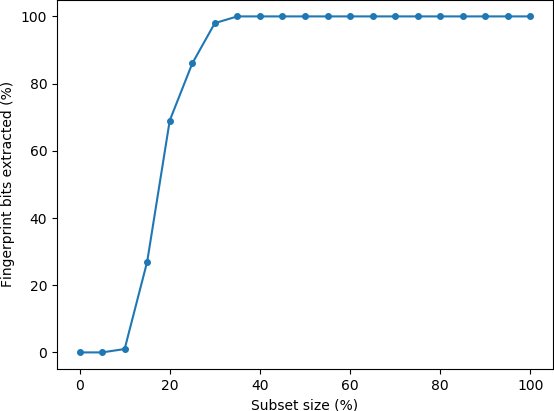
\includegraphics[width=6.7cm]{Figures/subset_attack_two-level_gamma100.png} }}
    \qquad
    \subfloat[$\gamma_1=50$]{{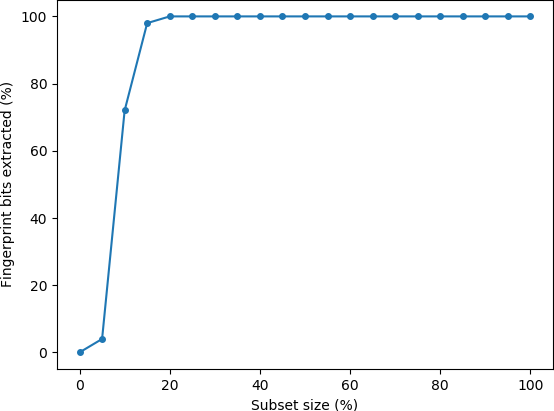
\includegraphics[width=6.7cm]{Figures/subset_attack_two-level_gamma50.png} }}
    \caption{Fingerprint extraction in a subset attack}
    \label{fig:subset-attack-two-level-fp-bits}
\end{figure}

The attack may cause that the extraction process does not manage to extract all the fingerprint bits correctly.
We can see from \Cref{fig:subset-attack-two-level-fp-bits}(a) that even if only around 35\% of the tuples are released by the malicious buyer, all fingerprint bits are still correctly extracted. 
The robustness of this scheme can be improved by changing the value of $\gamma_1$. 
\Cref{fig:subset-attack-two-level-fp-bits}(b) shows the results for a smaller $\gamma_1$, i.e. for the increased number of marks in the data that can be used to verify the ownership. 
For this parameter setting, the scheme is more robust against the subset attack, and even from only 20\% of the data, all the correct fingerprint bits can be extracted. 
For this experiments, we used the fingerprint of length $L=96$ and the bit significance level of each bit $\alpha_2$ is 0.01 (the confidence level is 99\%).

\begin{table}[ht]
    \centering
    \caption{Success of the subset attack on Two-level Fingerprinting Scheme}
    \label{tab:subset-attack-two-level}
    \begin{tabular}{|c|c|c|c|c|c|c|}
        \hline
         & $p'=60\%$ & $p'=70\%$ & $p'=80\%$ & $p'=90\%$ & $p'=95\%$ & $p'=99\%$ \\
         \hline
         $\gamma_1 = \gamma_2 = 10$ & 0 & 0 & 0 & 0 & 0 & 1.0 \\
         \hline
         $\gamma_1 = \gamma_2 = 25$ & 0 & 0 & 0 & 0.04 & 1.0 & 1.0 \\
         \hline
         $\gamma_1 = \gamma_2 = 50$ & 0 & 0 & 0.04 & 0.98 & 1.0 & 1.0 \\
         \hline
         $\gamma_1 = \gamma_2 = 100$ & 0 & 0.74 & 1.0 & 1.0 & 1.0 & 1.0 \\
         \hline
         $\gamma_1 = \gamma_2 = 200$ & 1.0 & 1.0 & 1.0 & 1.0 & 1.0 & 1.0 \\
         \hline
    \end{tabular}
\end{table}

Let us consider the setting where $\gamma_1=50$ and $\gamma_2=50$. For $p<20\%$ ($p'>80\%$; the attacker removes more than 80\% of the tuples) some bit positions will be unknown. For $p=15\%$ on average 2 out of 96 bit positions cannot be detected, creating $2^2$ fingerprint candidates. 
The fingerprint verification process may still select the correct fingerprint out of $2^2$ possible ones and the extraction algorithm finds the malicious buyer successfully. 
In the same setting, when 90\% of the tuples are removed, the algorithm correctly extracts 72\% correct fingerprint bits, or 69 out of 96. 
This is not enough for the fingerprint verification algorithm to verify any fingerprint and the detection algorithm fails. 
See the \Cref{tab:subset-attack-two-level} where the success of the subset attack is recorded. 
The experiments are run using Forest Cover Type data. 
The results in the table confirm that although not all fingerprint bits are extracted, the attack is not 100\% successful. 

\begin{figure}
    \centering
    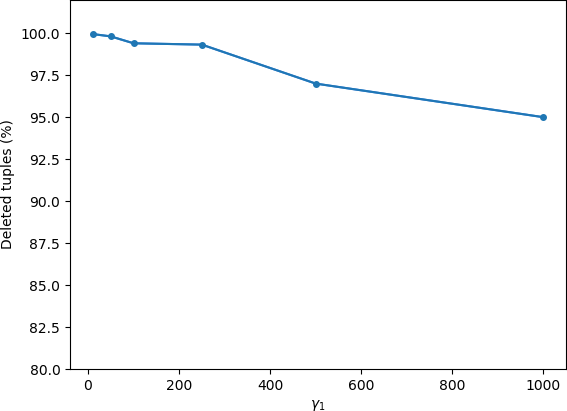
\includegraphics[width=0.7\textwidth]{Figures/subset_attack_two-level-ownership-ver.png}
    \caption{Ownership verification in a subset attack}
    \label{fig:subset-attack-ownership-verification}
\end{figure}

The first level of the embedding process provides the ownership verification even for cases when the correct fingerprint cannot be extracted. 
So, although the owner cannot trace the source of unauthorised leakage of data, she can claim the ownership. The mark created in this process is very robust. See in the \Cref{fig:subset-attack-ownership-verification} that even from the very small percentage of the data (<5\%), the detection algorithm will verify the owner with confidence level 99\% ($\alpha_1=0.01$).
The experiments are run even for the very big values of $\gamma_1$. 
For the settings where our experiments show high probabilities of extracting the right fingerprint from the small chunks of data, i.e $10<\gamma_1,\gamma_2<100$, up to 99\% of the tuples can be deleted and ownership can still be claimed.      

\subsection{Fingerprinting scheme for categorical data}
The fingerprinting scheme for categorical data complements the AK Scheme and for subset attack, we can refer to \Cref{eq:subset-attack-ak} as a starting point for analysis. 
The important difference between AK Scheme and scheme for categorical data is the introduction of modulo operation as one of the steps. 
We mentioned before in \Cref{subsec:fingerprinting-scheme-categorical} that we trade the strength of detection algorithm for fingerprinting categorical data successfully. 
This means that additional modulo operation step in the fingerprint insertion phase causes errors in the detection phase that cannot be avoided. 
Having errors in unaffected fingerprinting scheme increases the vulnerability of the scheme to attacks. 
Therefore, the \Cref{eq:subset-attack-ak} lacks influence of modulo operation in order to be credible. 
\Cref{tab:subset-attack-adult} shows the theoretical success of the subset attack on the dataset with $\eta = 30,162$ rows (convenient for comparison to experimental results on Adult dataset) if the effects of modulo are not taken into account, using \Cref{eq:subset-attack-ak}.
$\omega_i$ is approximated to $\eta/(\gamma*L)$ and $L=80$. 
Value 0 represents the perfect resistance to the subset attack, and 1 is the perfect success of the subset attack, i.e. the scheme completely failing to defend against it.

\begin{table}[ht]
    \centering
    \caption{Theoretical success rate of a subset attack on the fingerprinting scheme for categorical data, using the Adult data}
    \label{tab:subset-attack-adult}
    \begin{tabular}{|c|c|c|c|c|c|c|}
         \hline
        & \textbf{$p'=30\%$} & \textbf{$p'=60\%$} & \textbf{$p'=80\%$} & \textbf{$p'=90\%$} & \textbf{$p'=95\%$} & \textbf{$p'=99\%$}\\
        \hline
        $\gamma=3$ & 0.0 & 0.0 & 0.0 & 0.0001 & 0.1174 & 1.0 \\
        \hline
        $\gamma=6$ & 0.0 & 0.0 & 0.0001 & 0.0996 & 0.9601 & 1.0 \\
        \hline
        $\gamma=12$ & 0.0 & 0.0 & 0.0762 & 0.9555 & 1.0 & 1.0 \\
        \hline
        $\gamma=25$ & $1.15\times10^{-6}$ & 0.3166 & 0.9430 & 1.0 & 1.0 & 1.0 \\
        \hline
        $\gamma=50$ & 0.0052 & 0.7421 & 1.0 & 1.0 & 1.0 & 1.0 \\
         \hline
        $\gamma=100$ & 0.4783 & 0.9999 & 1.0 & 1.0 & 1.0 & 1.0 \\
         \hline
     \end{tabular}
\end{table}

\paragraph{Experiments}
The experiments are made on the Adult dataset as it is the dataset containing categorical attributes. 
We measure the success of subset attack over 500 runs and parameters set as follows: $L=80$, $\xi=1$, $\tau=0.5$, $\gamma=\{3,6,12,25,50,100\}$ and $p'=\{0.30,0.60,0.80,0.90,0.95,0.99\}$, where $p'$ represents the percentage of tuples that are deleted.


\begin{table}[ht]
    \centering
    \caption{Experimental results of the subset attack success rate on the fingerprinting scheme for categorical data, using the Adult data}
    \label{tab:subset-attack-adult-experimental}
    \begin{tabular}{|c|c|c|c|c|c|c|}
         \hline
        & \textbf{$p'=30\%$} & \textbf{$p'=60\%$} & \textbf{$p'=80\%$} & \textbf{$p'=90\%$} & \textbf{$p'=95\%$} & \textbf{$p'=99\%$}\\
        \hline
        $\gamma=3$ & 0.0 & 0.0 & 0.0 & 0.004 & 0.22 & 1.0 \\
        \hline
        $\gamma=6$ & 0.08 & 0.18 & 0.20 & 0.354 & 0.954 & 1.0\\
        \hline
        $\gamma=12$ & 0.078 & 0.0 & 0.212 & 0.97 & 1.0 & 1.0 \\
        \hline
        $\gamma=25$ & 0.012 & 0.284 & 0.99 & 1.0 & 1.0 & 1.0 \\
        \hline
        $\gamma=50$ & 0.346 & 1.0 & 1.0 & 1.0 & 1.0 & 1.0 \\
         \hline
        $\gamma=100$ & 0.976 & 1.0 & 1.0 & 1.0 & 1.0 & 1.0 \\
         \hline
     \end{tabular}
\end{table}

\Cref{tab:subset-attack-adult} and \Cref{tab:subset-attack-adult-experimental} share the same parameter settings for calculating the success of a subset attack on the Adult dataset, however, in latter the rate of success is larger overall.
Although the detection algorithm can detect the correct fingerprint from the full set of tuples, the errors introduced by modulo operation are enhancing the success of the attack. 
Therefore, only for small values of $\gamma$, the scheme is resistant to subset attack if the large portion of tuples is not deleted. 




\section{Superset attack}\label{subsec:superset-attack}

In a superset attack, an attacker adds additional tuples to the fingerprinted data, creating a bigger, pirated dataset.
This attack considers only the addition of the new tuples while the original set of tuples remains in the pirated dataset.
The sources of the additional tuples can be various.
One can add the tuples from other sources such as related datasets with similar attributes, artificial tuples with some semantic meaning, tuples generated from the dataset itself, or the values can be completely random. 
This attack can only be applied on fingerprinting schemes whose defence algorithms can and do function without the access to the original dataset (e.g. AK Scheme).
Otherwise, it is trivial to compare the pirated dataset to the original and remove the tuples that are added by an attacker.


Defence in some cases can be helped by syntactical examination of the dataset. 
In cases where additional tuples are generated completely randomly, it might be easy for a human to spot and remove them without any algorithm.
Also, any semantic background that the defence knows about the database can serve as the preliminary step in the deletion of additional tuples.


\subsection{AK Scheme}\label{subsec:superset-attack-ak}
Assume that fingerprint bit $f_i$ is embedded in the original data $\omega_i$ times, and that it is extracted from the additional tuples $\omega_i'$ times \cite{li2005fingerprinting}. 
Matching of the single extracted fingerprint bit to the correct value $f_i$ is modelled as an independent Bernoulli trial with probability 0.5 of success or failure.
(Extraction is controlled by the new unknown values of the primary key, therefore it is equally likely for the extracted bit to be 0 or 1.)
For the detection algorithm to fail in extracting the correct fingerprint bit, at least $(1-\tau)(\omega_i+\omega_i')$ embedded bits that correspond to the fingerprint bit $f_i$ must be detected wrongly.
Thus, the probability that the fingerprint is detected incorrectly is $B((1-\tau)(\omega_i+\omega_i');\omega_i',0.5)$.
The probability that the entire fingerprint is detected incorrectly is 
\begin{equation} \label{eq:superset-attack}
    fm = 1 - \prod_{i=0}^{L-1}(1-B((1-\tau)(\omega_i+\omega_i');\omega_i',0.5))
\end{equation}

Let us set $\tau=0.5$ (the usual default value) and analyse the performance of superset attack success for that case.
Knowing that all fingerprint bits will be correctly extracted from the original tuples because they are not changed, intuitively, in the tuples added by the attacker the incorrect occurrence of some fingerprint bit must outnumber its occurrences in the original tuples.
Formally, superset attack can be successful only if $\exists i\in\{0,...,L-1\}: \omega_i'\geq\omega_i$.
To make that possible, the attacker must add at least $100\%\eta$ tuples to the original data.

In AK Scheme the choice of fingerprint bit to be embedded is made randomly and independently in each step, therefore we can assume $\omega_i\approx\omega_j, \forall i,j \in \{0,...,L-1\}, i \neq j$. 
Furthermore, we can also assume $\omega_i'\approx\omega_j', \forall i,j \in \{0,...,L-1\}, i \neq j$.
\Cref{tab:superset-attack-forest} shows the success of the superset attack depending on $\gamma$ and number of added tuples. 
The success is calculated using \Cref{eq:superset-attack}, taking into account the assumptions made above. 
We analyse the success of superset attack for Forest Cover Type data with $L=96$ and $\tau=0.5$
Value 0 is the complete failure of the attack and 1 maximum success. 

\begin{table}[ht]
    \centering
    \caption{Superset attack success rate on the Forest Covertype data}
    \label{tab:superset-attack-forest}
    \begin{tabular}{|c||c|c|c|}
    \hline
         $\omega_i'$ & $\gamma=25$ & $\gamma=50$ & $\gamma=100$ \\
        \hline
         $100\%(\omega_i)$ & $1.35835\times10^{-71}$ & $3.61112\times10^{-35}$ & $8.32668\times10^{-17}$ \\
         \hline
         $200\%(\omega_i)$ & $1.91325\times10^{-27}$ & $8.66310\times10^{-14}$ & $1.81092\times10^{-6}$ \\
         \hline
         $300\%(\omega_i)$ & $8.32595\times10^{-18}$ & $9.89990\times10^{-9}$ & $0.000439$ \\
         \hline
         $400\%(\omega_i)$ & $3.31239\times10^{-13}$ & $1.55168\times10^{-6}$ & 0.006221 \\
         \hline
         $500\%(\omega_i)$ & $1.74078\times10^{-10}$ & 0.000047 & 0.029978 \\
         \hline
         $1000\%(\omega_i)$ & 0.000045 & 0.019113 & 0.536146 \\
         \hline
    \end{tabular}
\end{table}

The ratio $\omega_i/\omega_i'$ is approximately the same as ratio $\eta/\eta'$, where $\eta'$ is the number of added tuples because of the randomness in embedding the fingerprint, so we can interpret the percentages in the first row of \Cref{tab:superset-attack-forest} as the amount of added tuples in with respect to the original number of tuples. 

The success rates in the \Cref{tab:superset-attack-forest} are very small even for cases with a big number of added tuples, i.e. the scheme is very resilient to superset attack. 
Adding a lot of "fake" tuples to the dataset, in this case even several times more than the original dataset size, violates the credibility of the data. 
The attacker does not benefit from such attack, so the subset attack is usually combined with some other attack such as subset attack (\textit{mix-and-match} attack \cite{li2005fingerprinting}). 

\paragraph{}
Superset attack requires the generation of new "fake" rows which can be achieved in several ways. 
The attacker might come up with brand new values and combine them into new tuples or use the existing ones. 
In any case, the semantic problem might arise if the new values, or a combination of them, do not contextually fit the attribute or the dataset. 
For example, assume we have a dataset with information about persons such as their age, weight, height, etc. 
Generating new tuples might result in having tuples with illogical values for attributes, for example \textit{height}:240cm or a same person with values \textit{age}:10y. and \textit{height}:190cm.
In this case, the defence against the attack might be trivial, only by removing such tuples from the pirated dataset. 

One possible superset attack model consists of generating new tuples from the existing fingerprinted data and mixing those with the original fingerprinted data to create a pirated dataset.
The tuples are generated such that every attribute value (except for the private key) is independently randomly chosen from the set of existing values for that attribute.
This way we make it harder for a human to distinguish between the tuples originating from the originally fingerprinted data and those added by the attacker, making the defence rely entirely on detection algorithm.
The example of tuple generation is shown in \Cref{table:superset-attack-tuple-gen}.
The original tuples from which the values are generated are singled out and the sampled values are highlighted.
In the last row, we can see the generated tuple.


\begin{table}[ht]
\centering
\caption{Example of tuple generation}
\label{table:superset-attack-tuple-gen}
\resizebox{\textwidth}{!}{
\renewcommand{\arraystretch}{1.4}
\begin{tabular}{|c|c|c|c|c|c|c|c|c|c|c|c|} 
 \hline
 Id & El. & Asp. & Slope & HD-H & VD-H & HD-R & HS-9am & HS-noon & HS-3pm & HD-FP & C-Type\\
 \hline
 75 & 2864 & 118 & 18 & \textbf{\Large{201}} & 74 & 4567 & 248 & 221 & 93 & 4849 & \textbf{\Large{2}} \\
 \hline
 191 & 2995 & 173 & 15 & 268 & \textbf{\Large{135}} & 6312 & 228 & 246 & 146 & 4135 & \textbf{\Large{2}}\\
 \hline
 893 & 2924 & 270 & 10 & 134 & 11 & 5066 & 194 & 244 & \textbf{\Large{189}} & 1652 & 5\\
 \hline
 1258 & 2803 & \textbf{\Large{57}} & 32 & 323 & 136 & 342 & 223 & 157 & 45 & 1851 & 5\\
 \hline
 2165 & \textbf{\Large{3390}} & 59 & 10 & 124 & 12 & 2610 & 228 & 219 & 124 & 2357 & 7\\
 \hline
 6880 & 2983 & 297 & \textbf{\Large{11}} & 713 & -51 & 1543 & 190 & 237 & 186 & \textbf{\Large{2003}} & \textbf{\Large{2}}\\
 \hline
 11643 & 2911 & 332 & \textbf{\Large{11}} & 67 & 2 & 4972 & 193 & 225 & 172 & 1724 & 5\\
 \hline
 19210 & 2737 & 20 & 7 & 95 & 14 & \textbf{\Large{2314}} & 215 & 225 & 147 & 6815 & \textbf{\Large{2}}\\
 \hline
 23117 & 2877 & 165 & 3 & 30 & 4 & 5236 & \textbf{\Large{222}} & 240 & 154 & 4279 & 1\\
 \hline
 23135 & 2801 & 116 & 9 & 30 & 2 & 4709 & 236 & \textbf{\Large{231}} & 126 & 4807 & \textbf{\Large{2}}\\
 \hline
 \hline
 \large{581012} & \large{3390} & \large{57} & \large{11} & \large{201} & \large{135} & \large{2314} & \large{222} & \large{231} & \large{189} & \large{2003} & \large{2}\\
 \hline
\end{tabular}}
\end{table}

\subsection{Block Scheme}
Superset attack essentially does not work if the original dataset is available in the fingerprint detection process. 
Block Scheme detection algorithm requires the original dataset to extract the fingerprint as discussed in \Cref{subsec:block-oriented-scheme}, therefore this kind of attack alone, without a combination with some other attack does not make much sense.
The owner trivially removes the tuples from the pirated dataset that are not part of the original and proceeds with the detection algorithm.

\subsection{Fingerprinting scheme for the categorical data}
The blind, simplistic fingerprinting scheme described in \Cref{subsec:fingerprinting-scheme-categorical} behaves in the same way as the AK Scheme against the superset attack. Therefore, we refer to \Cref{subsec:superset-attack-ak}.

The second discussed scheme which is based on neighbourhood search is not blind. It means that any additional fake tuples in the dataset would easily be detectable and removed by a simple check and comparison with the original dataset.

\section{Bit-flipping attack}
The subset and superset attacks described in \Cref{subsec:subset-attack} and \Cref{subsec:superset-attack} respectively, are targeting the disruption of tuples without changing the values inside the dataset. 
However, the attacker might change values by selecting some bits and flipping their values in an attempt to destroy the fingerprint.
This kind of attack is called a bit-flipping attack.
The choice of the bits is random because the attacker is modelled such that he has no knowledge about the owner's secret key that is crucial for fingerprint insertion scheme.

\subsection{AK Scheme}
Let \textit{p} be the probability that the attacker flips some $k^{\text{th}}$ least significant bit, with $p \leq 0.5$ (otherwise fingerprint detection can be applied to transformed data by flipping each fingerprintable bit back). 
The attacker chooses bits independently, therefore bit flipping is modelled as an independent Bernoulli trial with probability \text{p} of success and $1-p$ of failure. 
Assume that each fingerprint bit $f_i$ is embedded $\omega_i$ times.
The detection algorithm will fail to extract the correct fingerprint bit if the correct bit value is extracted less than the defined number of times which is controlled by parameter $\tau$.
Therefore at least $(1-\tau)\omega_i$ embedded bits must be flipped by an attacker.
Thus, the probability that the fingerprint $f$ is detected incorrectly is
\begin{equation}\label{eq:fm-bit-flipping-ak}
    fm=1-\prod_{i=0}^{L-1}(1-B(\lfloor(1-\tau)\omega_i\rfloor;\omega_i,p))
\end{equation}

Because the choice of fingerprint bits to be embedded in fingerprint embedding process is completely random, we can assume that each fingerprint bit will be embedded in the data approximately same number of times; $\omega_0=\omega_1=...=\omega_{L-1}=\omega, \forall i, j \in \{1,L-1\}, i\neq j$.
Therefore, we can write the expression for false miss rate (\Cref{eq:fm-bit-flipping-ak}) as $fm = 1 - (1-B(\lfloor(1-\tau)\omega\rfloor;\omega,p))^L$.
The results in \Cref{table:bit-flipping-ak} and \Cref{table:bit-flipping-ak-tau} are obtained using this approximation of false miss rate. 
Since $0<B(\lfloor(1-\tau)\omega\rfloor;\omega,p)\leq1$, by increasing $L$ the false miss rate also increases, meaning that longer fingerprints lead to schemes more vulnerable to bit-flipping attack.
Intuitively, longer fingerprint means fewer embeddings of each single fingerprint bit in the data and larger probability for the attacker to erase all of the embeddings of some fingerprint bit, making the detection algorithm incapable of detecting a valid fingerprint. 

The effect of parameter $\gamma$ is shown in \Cref{table:bit-flipping-ak} by calculating probabilities of success of bit-flipping attack for different values of $\gamma$ and $p$ (probability of flipping a bit, i.e. the approximate amount of tuples containing a value with a flipped bit).
We choose $\gamma=\{6, 12, 25, 50, 100, 200\}$ and $p=\{45\%, 40\%, 30\%, 20\%\}$, and set $\tau=0.5$ and $L=96$ as fixed values.
$\omega$ is calculated as $\eta/(L*\gamma)$, and $\eta=581,012$ for the convenience of comparing these results to the experimental results on Forest Covertype dataset.

\begin{table}[ht]
\centering

\caption{Probability of a successful bit-flipping attack on the AK Scheme}
\label{table:bit-flipping-ak}
\begin{tabular}{|c|c|c|c|c|} 
 \hline
   & \textbf{$p=20\%$} & \textbf{$p=30\%$} & \textbf{$p=40\%$} & \textbf{$p=45\%$} \\
 \hline
 $\gamma=6$ & 0 & 0 & $6.6530 \times 10^{-9}$ & 0.0671 \\
 \hline
 $\gamma=12$ & 0 & 0 & 0.0003 & 0.7327 \\
 \hline
 $\gamma=25$ & 0 & $5.8392\times 10^{-9}$ & 0.0941 & 0.9987 \\
 \hline
 $\gamma=50$ & 0 & 0.0002 & 0.7144 & 1 \\
 \hline
  $\gamma=100$ & $2\times 10^{-5}$ & 0.0839 & 0.9994 & 1 \\
  \hline
  $\gamma=200$ & 0.0220 & 0.8060 & 1 & 1 \\
 \hline
\end{tabular}
\end{table}

The effect of parameter $\tau$ is shown in \Cref{table:bit-flipping-ak-tau}.
The success of the bit-flipping attack is calculated for different values of $\tau$ and $p$, while $L=96$ and $\gamma=50$ are set as fixed values.

\begin{table}[ht]
\centering
\caption{Probability of a successful bit-flipping attack on the AK Scheme}
\label{table:bit-flipping-ak-tau}
\begin{tabular}{|c|c|c|c|c|} 
 \hline
 & \textbf{$p=45\%$} & \textbf{$p=40\%$} & \textbf{$p=30\%$} & \textbf{$p=20\%$} \\
 \hline
 $\tau=0.50$ & 1 & 0.7144 & 0.0002 & 0 \\
 \hline
 $\tau=0.55$ & 1 & 0.9999 & 0.0228 & 0 \\
 \hline
 $\tau=0.60$ & 1 & 1 & 0.5779 & $2\times 10^{-5}$ \\
 \hline
 $\tau=0.65$ & 1 & 1 & 1 & 0.0048 \\
 \hline
  $\tau=0.70$ & 1 & 1 & 1 & 0.3041 \\
  \hline
  $\tau=0.75$ & 1 & 1 & 1 & 0.9996 \\
 \hline
\end{tabular}
\end{table}

Both $\tau$ and $\gamma$ affect the success of the attack such that if they are increased, the probability that fingerprint will not be detected correctly is also increased, i.e. the scheme is more susceptible to bit-flipping attack.
Generally, if the attacker chooses to flip more bits, i.e. increases $p$, that also increases his chance for the successful attack, but in the same time violates credibility of the data since more original values would be changed.
Note that parameter $\xi$ does not affect the success of the attack because it is not important which LSB of a chosen value is flipped by the attacker. 

\paragraph{Misattribution false hit}
Let us now analyse the probability of detecting valid but incorrect fingerprint caused by a bit-flipping attack - misattribution false hit $fh^A$.
The detection algorithm will extract a binary bit for fingerprinting bit $f_i$ if either at most $\lfloor(1-\tau)\omega_i\rfloor-1$ or at least $\lfloor\tau\omega_i\rfloor$ of its embedded bits are flipped.
If the detection algorithm extracts a binary string, the probability that the binary string is valid but belongs to an innocent buyer is $\frac{N-1}{2^L}$.
Therefore, the probability of detecting valid but incorrect fingerprint is 
\begin{equation} \label{missattribution-false-hit-ak-bit-flipping}
    fh^A=\frac{N-1}{2^L}\prod_{i=0}^{L-1}(1-B(\lfloor(1-\tau)\omega_i\rfloor;\omega_i,p)+B(\lfloor\tau\omega_i\rfloor;\omega_i;p)).
\end{equation}

\paragraph{}
False miss rate is by definition the sum of misattribution false hit and false negative rate.
Therefore, false negative is straightforward:

\begin{equation}
\begin{aligned}
fn=& 1-\prod_{i=0}^{L-1}(1-B(\lfloor(1-\tau)\omega_i\rfloor;\omega_i,p))- \\ & \frac{N-1}{2^L}\prod_{i=0}^{L-1}(1-B(\lfloor(1-\tau)\omega_i\rfloor;\omega_i,p)+B(\lfloor\tau\omega_i\rfloor;\omega_i;p)).
\end{aligned}
\end{equation}

\paragraph{Experiments}
We have run experiments on the Forest dataset and obtained results that are shown in table \ref{table:bit-flipping-ak-emp}. 
As it is shown in the previous section, the success of bit-flipping attack is influenced by multiple parameters - length of the fingerprint \textit{L}, fingerprint detection assurance parameter $\tau$, amount of marked values $\gamma$ (or equivalently, number of embedded bits corresponding to a single bit $\omega$) and the attacker's parameter \textit{p} that defines the number of flipped bits in pirated data. 
For our experiments we fix the values of $L=96$ and $\tau=0.5$.
We run 100 experiments with different random bit-flipping pattern for each of the combinations of parameters $\gamma = {6,12,25,50,100}$ and $p={20\%,30\%,40\%,45\%}$.

\begin{table}[ht]
\centering
\caption{Experimental results of a bit-flipping attack on the AK Scheme, using the Forest Cover Type data}
\begin{tabular}{|c|c|c|c|c|} 
 \hline
 & \textbf{$p=20\%$} & \textbf{$p=30\%$} & \textbf{$p=40\%$} & \textbf{$p=45\%$} \\
 \hline
 $\gamma=6$ & 0 & 0 & 0.50 & 0.56  \\
 \hline
 $\gamma=12$ & 0  & 0 & 0.50 & 1.0 \\ 
 \hline
 $\gamma=25$ & 0  & 0 & 0.54 & 1.0  \\
 \hline
 $\gamma=50$ & 0 & 0.50 & 0.72 & 1.0   \\
 \hline
  $\gamma=100$ & 0 & 0.86 & 1.0 & 1.0  \\
 \hline
\end{tabular}
\label{table:bit-flipping-ak-emp}
\end{table}

The experimental results show that flipping 40\% of the bits available for fingerprinting most likely deletes the fingerprint. At 30\% the schemes with bigger $\gamma$ ($\gamma=50,100)$, i.e. less embedded marks, fail under the bit-flipping attack. 
Generally, the scheme is more robust against the attack for a smaller value of $\gamma$.
The empirical results differ from the analytic results in \Cref{table:bit-flipping-ak}. The two analysis agree on the cases where the attack completely succeeds and completely fails, however, in our experiments the scheme appears less robust to the bit-flipping attack than it is suggested in the analysis. 
The success rates in \Cref{table:bit-flipping-ak} are calculated using \Cref{eq:fm-bit-flipping-ak} under the assumption that all fingerprint bits are embedded the same number of times, which is approximated with $\omega$. 
This is not true due to the random nature of bit choice. In reality, every fingerprint bit has it's own $\omega_i$ value. Many fingerprint bits, thus, are embedded in data less than $\omega$ times and are easier to destroy. Since destroying all occurrences of just one fingerprint bit makes the fingerprint impossible to extract, the low occurrences of some fingerprint bits might decrease the robustness. 
This might be the reason for the difference in the attack success rates. 
Even though the probabilities for attack success are different, the boundary for robustness is confirmed. 
For $\gamma=\{6,12,25\}$ it is safe to flip up to 30\% of LSBs to not remove the fingerprint, and for larger values, $\gamma=\{50,100\}$, it is safe to flip around 20\% of the LSBs.

\subsection{Block Scheme}
Assume that the attacker examines every bit available for fingerprinting independently and selects it for flipping with probability $p$.
Let us approximate the number of times that each fingerprint bit is embedded in the data to $\omega$.
For the detection algorithm to fail to recover the correct fingerprint bit, at least $(1-\tau)\omega$ embedded bits corresponding to the single fingerprint bit $f_i$ must be changed, i.e. more than $\omega - \lceil\tau\omega\rceil+1$ bits must be changed.
Probability that one fingerprint bit is destroyed is $B(\omega-\lceil\tau\omega\rceil+1;\omega,p)$.
The probability that the entire fingerprint will be detected incorrectly is therefore 
\begin{equation}
    fm=1-(1-B(\omega-\lceil\tau\omega\rceil+1;\omega,p))^L
\end{equation}

Table \ref{table:bit-flipping-block} shows the probabilities that the bit-flipping attack will be successful on Block Scheme, depending on $p$ and $\beta$.
Parameters are set as follows: $\xi=2$, $\tau=0.5$ and $L=96$.
We choose $\eta=581012$ and $v=10$, same as Forest Covertype dataset. 

\begin{table}[ht]
    \centering
    \caption{Probability of a successful bit-flipping attack on the Block Scheme}
    \label{table:bit-flipping-block}
    \begin{tabular}{|c|c|c|c|c|}
    \hline
         & p=30\% & p=40\% & p=45\% & p=50\%\\
         \hline
        $\beta=5$ & 0 & 0 & 0 & 1.0 \\
        \hline
        $\beta=10$ & 0 & 0 & 0.02 & 1.0 \\
        \hline
        $\beta=15$ & 0 & 0.002 & 0.88 & 1.0 \\
        \hline
        $\beta=20$ & 0 & 0.017 & 0.97 & 1.0 \\
        \hline
    \end{tabular}
\end{table}


\paragraph{Experiments}
We run experiments on the Forest dataset with the previously defined parameters.
Table \ref{table:bit-flipping-block-emp} shows the obtained empirical results for the success of the bit-flipping attack on the Block Scheme.
Each experiment is run 100 times and the table shows the average success of the bit-flipping attack. 

\begin{table}[ht]
    \centering
    \caption{Experimental results of the bit-flipping attack on the Block Scheme, for the Forest Cover Type data}
    \begin{tabular}{|c|c|c|c|c|}
    \hline
         & p=30\% & p=40\% & p=45\% & p=50\%\\
         \hline
        $\beta=5$ & 0 & 0 & 0.50 & 1.0 \\
        \hline
        $\beta=10$ & 0 & 0.50 & 0.50 & 1.0 \\
        \hline
    $\beta=15$ & 0 & 0.50 & 0.92 & 1.0 \\
        \hline
        $\beta=20$ & 0.08 & 0.50 & 1.0 & 1.0 \\
        \hline
    \end{tabular}
    \label{table:bit-flipping-block-emp}
\end{table}

The experiments confirm the rule that having more marks in the data, i.e. smaller $\beta$, makes the scheme more robust against the bit-flipping attack.
Our experimental rates of the attack success, however, differ from the analytical results in \Cref{table:bit-flipping-block}. 
The change might be due to the implementation limitations introduced by the design of the Block Scheme. 
We address in \Cref{subsec:assumptions-block} the problem of "extra data" that in reality never gets fingerprinted.
This means that less data is fingerprinted, i.e. fewer marks are in the data due to this limitation than it is assumed for the calculation of the theoretical attack success rates.
This might be the reason why experimentally this scheme appears to be more vulnerable to the attack than expected by the theoretical analysis.

The scheme with all of the chosen parameters guarantees robustness for to 30\% flipped LSBs. Choosing a small value of $\beta$, e.g. 5, the tolerated amount of flipped bits rises up to 45\%.
We can argue that this is indeed a robust scheme. The assumed attacker would like to keep the data useful, and flipping more bits significantly changes the values in the data and the utility decreases.


\subsection{Two-level Fingerprinting Scheme}
In this section, we empirically analyse the robustness of the Two-level Fingerprinting Scheme against the bit-flipping attack. 
We measure the success on two levels; the ownership verification and the fingerprint extraction.
The attacker might be able to either (i) disable both ownership verification and fingerprint extraction, (ii) destroy the fingerprint but fail in disabling ownership verification, or (iii) fail in both. 
We use the Forest Covertype data for the experiments and measure success of the subset attack over 500 runs of each parameter setting. We choose: $L=96$, $\xi=2$, $\alpha_1=\alpha_2=\alpha_3=0.01$, $\gamma_1=\gamma_2=\{10,25,50,100\}$.
\Cref{fig:bit-flip-two-level-fp} shows the results of the experiments.

\begin{figure}[ht]
    \centering
    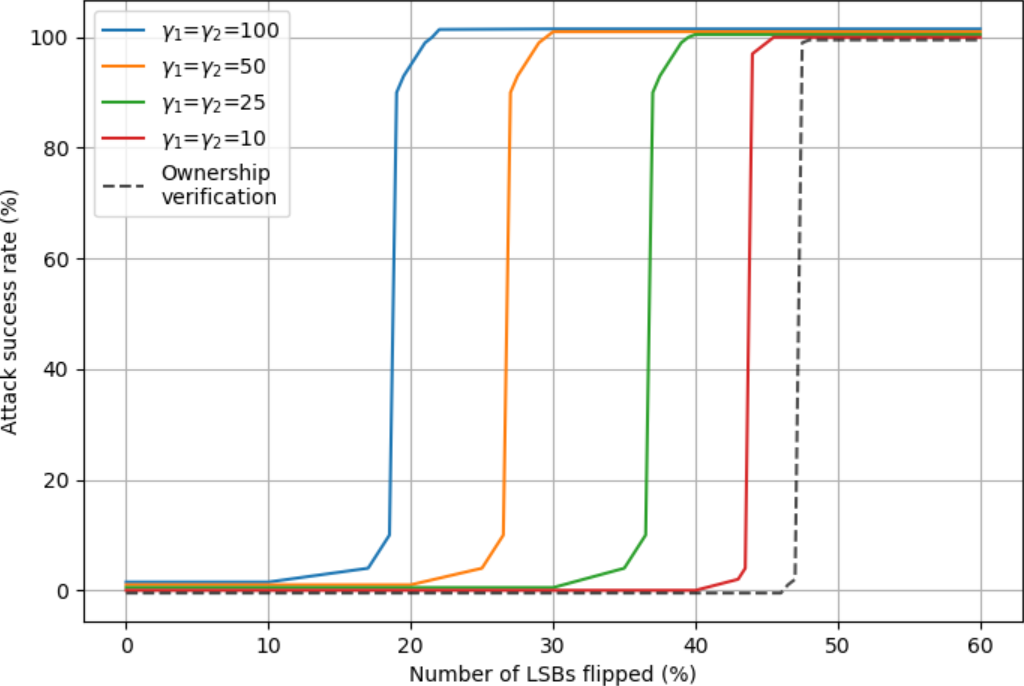
\includegraphics[width=0.9\textwidth]{Figures/bit-flip-two-level-screensh.png}
    \caption{Bit-flipping attack success in the Two-level Fingerprinting Scheme}
    \label{fig:bit-flip-two-level-fp}
\end{figure}

The coloured lines show the success rate of the attacks against the fingerprint extraction. 
The dashed line shows the success rate of the attack against the ownership verification.
The experiments show that the robustness against the bit-flipping attack, as expected, grows with more embedded marks.
The scheme with $\gamma_1=\gamma_2=100$ fails to extract the fingerprint when 19\% of the LSBs are flipped by the attacker, while the scheme with $\gamma_1=\gamma_2=10$ fails at approximately 43\% flipped LSBs.
In both cases, the ownership is verified 100\% of the times, even though the exact fingerprint cannot be extracted. 
The ownership verification fails with approximately 47\% flipped LSBs. 
The robustness of the ownership verification is very similar for each $\gamma_1$ value, therefore we represent it with only one (dashed black) line in \Cref{fig:bit-flip-two-level-fp}.

Choosing smaller $\gamma$ values makes the Two-level Fingerprinting Scheme very robust against the bit-flipping attack. The two-level fingerprint provides the additional protection measure of verifying the ownership even in cases when the exact fingerprint cannot be extracted. 
Smaller values of $\gamma$, however, introduce more error in data. How these errors affect the utility of the data, we discuss in \Cref{chapter:Utility}.

\section{Additive Attack}
Consider a scenario where the attacker tries to claim the ownership of the dataset by inserting an additional fingerprint in the bought dataset. We call this strategy an additive attack \cite{agrawal2003watermarking}. The competing ownership claims can be resolved if there exists at least one bit that both the owner and the attacker have marked, each with a different value. The way to resolve the ownership claim competition is to determine which owner's marks win, i.e. which mark has overwritten the other. The winning owner's mark is clearly inserted later, therefore his claim of ownership is false.

Method for dealing with the false claims of ownership could be to ask both the owner and the attacker to produce the original dataset before it was fingerprinted and to demonstrate the presence of the fingerprint in each other's original datasets. 
The owner will be able to demonstrate the presence of her fingerprint in the attacker's original unlike the attacker in the owner's original. 


\subsection{AK Scheme}\label{subsubsec:additive-ak}
In the AK Scheme, it is justified to conclude that the odds of finding such conflicting bits are low. 
Suppose that the data fingerprinted by the owner is marked $\omega$ times with parameters $\gamma$, $v$ and $\xi$ and that the attacker performs the fingerprinting insertion algorithm with parameters $\gamma'$, $v'$ and $\xi'$. Under the usual probabilistic model of AK Scheme's bit-marking process, the probability that a specified bit marked by original fingerprint is also marked by the attacker is the product of probabilities that the tuple containing the bit is chosen for marking $(1/\gamma')$, that the attribute containing the bit is also chosen for marking $(1/v')$ and that the specified bit is chosen $(1/\xi')$. The probability that the attacker's mark is different from the original mark is 1/2 so that the overall probability that the specified bit is a conflict bit is $1/(2\gamma'v'\xi')$. The tuples are marked independently of each other, therefore the probability that the attack is successful, i.e. no conflicting bits are found, is
\begin{equation}
    P\{success|\omega\}=(1-\frac{1}{2\gamma'v'\xi'})^\omega
\end{equation}

For example, let the dataset have around 500,000 tuples and  $\omega=1000$. 
Assume that attacker wants to increase his chances of success.
If the attacker sets $\gamma'=10,000$ (a rather big value considering that it means that only 1/10,000 tuples will be marked), $v'=10$ and $\xi'=5$, then $P\{success|\omega\}=(1-10^{-6})^1000 \approx 0.999$.



\subsection{Block Scheme}
The solution from section \ref{subsubsec:additive-ak} is applicable to the block fingerprinting scheme as well. 
Suppose that the attacker runs the fingerprint insertion algorithm with parameters $\beta'$, $\xi'$ and $v'$.  
Let $1/\gamma'$ be the percentage of tuples marked by the attacker.
Due to the uniform distribution of the marks in the Block Scheme, we can approximate the percentage $1/\gamma \approx (\xi v)/\beta^2$, assuming that there is in average no more than 1 mark in a single tuple.
Let the data be marked $L\omega$ times in total by the owner.
The probability that the additive attack is successful is then 

\begin{equation}
\begin{aligned}
    P\{success|L\omega\}&=(1-\frac{1}{2\gamma'v'\xi'})^{L\omega} \\
        &=(1-\frac{1}{2\frac{\beta'^2}{\xi'v'}v'\xi'})^{L\omega} \\
        &=(1-\frac{1}{2\beta'^2})^{L\omega}
\end{aligned}
\end{equation}

The success of the additive attack depends exponentially on $L\omega$.
The attacker can increase his chances for success by increasing $\beta'$, however with $L\omega \gg \beta'$, the chances for the successful attack are low.
For example, with $\beta'=30$ and $L\omega=10000$, $P\{success|L\omega\}=0.0039$.



\section{Collusion Attack} \label{subsec:collusion}

Fingerprinting produces distinct copies of the data for each of the buyers. 
This opens the possibility for multiple buyers to have access to each other's copies of the data, all fingerprinted with different fingerprints, and work in coalition in order to create a useful data copy that would not implicate any member of the coalition. 
One possibility for the members of the coalition is to attempt to erase the fingerprint or to modify values such that detection algorithm implies an innocent buyer who is not a member of the coalition to be the traitor.
Collusion attack is specific for fingerprinting, as opposed to other attacks discussed in this thesis that can be applied in the context of watermarking. 
Collusion is studied extensively in the literature \cite{boneh1998collusion, guth1999error, pfitzmann1999coin, pfitzmann1996asymmetric, yacobi2001improved} and collusion resistant fingerprinting codes have been proposed such as one by Blakley et al. \cite{blakley1985fingerprinting}, by Guth and Pfitzmann \cite{blakley1985fingerprinting}, and probably the most well-know by Boneh and Shaw - \textit{BoSh} \cite{boneh1998collusion}.

Boneh and Shaw \cite{boneh1998collusion} provide the definitions of collusion-secure codes and propose the methods for construction of codes and algorithm for dealing with collusion attacks. 
The method can be used for fingerprinting any sort of digital data: documents, multimedia, software, etc. 
The effectiveness of the approach is based on the \textit{Marking Assumption} that states that "the main property of the marks should be satisfied are that users cannot change the state of an undetected mark without rendering the object useless" \cite{boneh1998collusion}. The colluding buyers can detect only the fingerprint bits in which their copies differ, otherwise, the fingerprint cannot be detected. 
For instance, two buyers with their fingerprinted dataset can fairly easily compare their datasets and remove or change the values that differ between the copies.

The following definitions of collusion-secure codes are defined \cite{boneh1998collusion}:
\begin{itemize}
    \item \textbf{$c$-frameproof code} satisfy that no coalition of at most \textit{c} members can frame a user who is not part of the coalition. $c$-frameproof codes prevent this harder version of treason but do not assure that the traitor(s) will be found
    
    \item \textbf{totally $c$-secure code} is a code for which exist an algorithm that outputs a member of a coalition with at most $c$ members that generated an arbitrary code under the coalition. It is proven that for $c \geq 2$ the totally c-secure code does not exist.
    
    \item \textbf{$c$-secure code with $\epsilon$-error} is a relaxation of the previous - if the code is $c$-secure with $\epsilon$-error, then there exists an algorithm which outputs a member of coalition with at most $c$ members with probability $1-\epsilon$, $\epsilon \in [0,1]$. 
\end{itemize}

BoSh codes are designed to be $c$-secure with $\epsilon$-error. 
Increasing $c$ or reducing $\epsilon$ provides better security definition, but results in longer codes.
BoSh code is generated as a concatenation of $b$ code-words of size $(a-1)d$ from public "inner code" that is common for all buyers. 
Therefore, the code has length $b(a-1)d$.
Code words from the inner code are chosen according to the secret buyer-specific "outer code" and randomly permuted before the use. 
$a$, $b$ and $d$ are code construction parameters (in \cite{boneh1998collusion} $n$, $L$ and $d$ respectively, but we change the notation due to overlapping with notation in this thesis).
The parameter values are: $a=2c$, $b=2c\log(2N/\epsilon)$ and $d=2a^2 \log(4ab/\epsilon)$.
It is required that the random permutation and random outer code for each buyer are kept secret from all buyers.
The tracing algorithm takes as input pirated data under collusion attack and returns exactly one malicious buyer. 

\paragraph{AK Scheme}
AK insertion algorithm (\Cref{alg:AK-insertion}) is not secure against collusion attack. 
Each fingerprint bit $f_i$ is embedded to the same place in every fingerprinted copy of the dataset since it only depends on parameters $\gamma$, $v$ and $\xi$ which are not buyer-specific, and owner's secret key $\mathcal{K}$.
Assume that 3 buyers are in collusion and they extract following marks from the bits that differ within their copies: (1,0,1), (1,1,0) and (0,1,1). 
They decide to change values according to the majority, so they come up with the new mark (1,1,1) that they use to create the pirated data. 
Detection algorithm cannot match the new fingerprint to any of the members of the coalition. 
Another option for members of the collusion is to produce a random mark, e.g. (0,0,1) which leads to the same outcome. 

To create a collusion-resistant scheme, authors in \cite{li2005fingerprinting} propose the modified version of BoSh code that is adequate to be incorporated into AK Scheme. 
The fingerprint in the proposed solution consists of two parts: (1) watermark which is the same for every buyer and computed from a hash function using owner's secret key, $\mathcal{H}(\mathcal{K})$, and (2) BoSh code. 
Those two parts are concatenated to create the fingerprint.

There are two main differences between BoSh code and proposed solution \cite{li2005fingerprinting}:
\begin{enumerate}
    \item Collusion-resistant AK Scheme does not require recording of secret outer code for every buyer as it is the case for BoSh codes. Storing any kind of secret buyer-specific information is already discussed to violate key-based property and as a reason for incorporating pseudo-random sequence generator in the context of a fingerprint. The outer code needs to be hidden from the buyers, but deterministic to the owner. Therefore, the outer code is in collusion-resistant AK Scheme generated using such pseudo-random sequence generator from the owner's secret key $\mathcal{K}$ and buyer's ID number.
    
    \item Similarly, the random permutation for all buyers needs to be stored in BoSh code setting. The purpose of the final random permutation in BoSh code is to hide which mark in dataset corresponds to which fingerprint bit. In AK Scheme this permutation is not necessary as the choice of fingerprint bit to be embedded is already random by the design of the insertion algorithm (lines 7 and 8 in \Cref{alg:AK-insertion}).
    
\end{enumerate}

Insertion and detection algorithms of collusion-resistant AK Scheme are slightly modified insertion (\Cref{alg:AK-insertion}) and detection (\Cref{alg:AK-detection}) algorithms of AK. 
The modifications in the insertion algorithm are as follows:
\begin{enumerate}
    \item Additional parameter $L_1$ represents the length of the first (watermarking) part of a fingerprint. $L=L_1+L_2$ ($L_2$ is the length of second part - BoSh code).
    \item Generation of fingerprint replaced by concatenation of watermark part of the fingerprint and BoSh code.
    \item Additional parameter $c$ - maximum coalition size
    \item Additional parameter $\epsilon$ - maximum false detection rate in tracing a coalition
\end{enumerate}
The detection algorithm is modified such that it runs in two consecutive phases:
\begin{enumerate}
    \item \textbf{Watermark check} - in this part, the watermark part $\mathcal{F_1}$ of recovered fingerprint template $\mathcal{F}$ is checked against the inserted codeword. The algorithm returns \textit{none suspected} for a single bit mismatch. This phase serves as prevention from 100\% misdiagnosis false hit rate in cases where non-pirated data is the input of detection algorithm (because the following phase returns exactly one malicious buyer). 
    \item \textbf{BoSh tracing algorithm} (from \cite{boneh1998collusion}) - if algorithm passes the first phase, this phase identifies exactly one malicious buyer.
\end{enumerate}

Authors of \cite{li2005fingerprinting} analyse the robustness rates of collusion-resistant AK Scheme and carry out the experimental results on scheme robustness.
Following the proof from \cite{boneh1998collusion} that probability of BoSh tracing algorithm returning the buyer who is indeed a member of the coalition is greater than $1-\epsilon$, the false miss rate $fm$ and misattribution false hit $fh^A$ satisfy
\begin{equation}
    fm=fh^A \leq \epsilon
\end{equation}
The misdiagnosis false hit $fh^D$ when the detection algorithm is applied on unmarked dataset is
\begin{equation}
    fh^D=\prod_{i=0}^{L_1-1}B(\lfloor\tau\omega_i\rfloor;\omega_i,0.5)\leq \frac{1}{2^{L_1}})
\end{equation}
and it can be decreased exponentially by increasing $L_1$ ($fh^D \simeq0$ if $L_1 \gg 1$).


\section{Summary}
In this chapter, we analysed the robustness of the fingerprinting techniques under certain types of attacks. We address subset attack, superset attack, bit-flipping attack, additive attack and collusion attack. 
As opposed to analysing the inability of a scheme to detect the fingerprint under a malicious attack, we also address the possibility of detecting the fingerprint in unmarked data - misdiagnosis false hit.

%misdiagnosis
\begin{figure}[ht]{
    \centering
    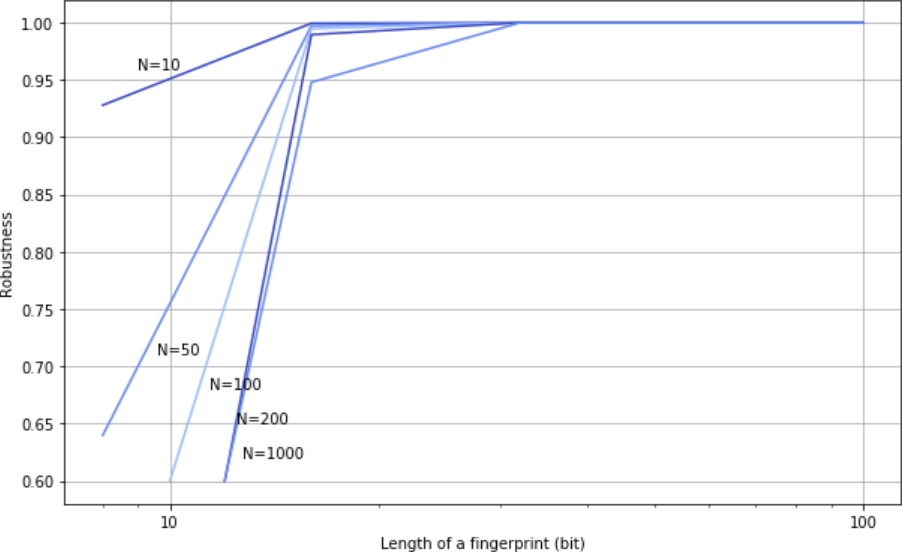
\includegraphics[width=0.8\textwidth]{Figures/misdiagnosis.PNG}
    \caption{Misdiagnosis false hit rate}
    \label{fig:misdiagnosis}
 }   
 \end{figure}

To avoid the misdiagnosis false hit, the fingerprint length must be big enough. \Cref{fig:misdiagnosis} shows the robustness of a scheme given the assumed number of buyers. We see that for the larger number of buyers we must ensure the longer fingerprint, e.g. if there are 100 buyers, the fingerprint length $L$ should be larger than 30.
 
The additive attack is, like misdiagnosis false hit, not specific for a certain scheme. The robustness of the scheme against the additive attack depends on the number of marks the scheme embeds in the data, which is controlled by parameters $\gamma$ in AK Scheme and the Scheme for fingerprinting categorical data, by $\gamma_1$ and $\gamma_2$ in Two-level Scheme and by $\beta$ in the Block Scheme.
%additive
\begin{figure}{
    \centering
    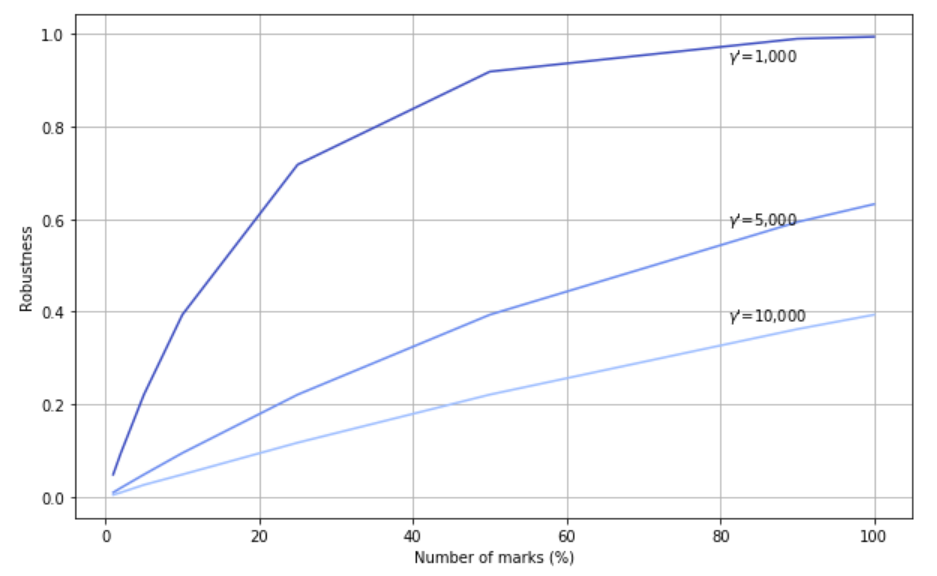
\includegraphics[width=0.8\textwidth]{Figures/additive.PNG}
    \caption{Robustness against the additive attack}
    \label{fig:additive-attack}
}\end{figure}
%subset
We show in \Cref{fig:additive-attack} the relation between number of marks and robustness of the scheme for different attacker's embedding patterns. 
The attacker's parameter of the ratio of the marked tuples is $\gamma'$ ($\gamma'=1,000$ means that one in a thousand tuples is marked). 
It depends on the attacker how he chooses to embed his fake fingerprint. If the dataset is very big and marking one in 10,000 tuples is sufficient to claim his ownership, then the fingerprinting schemes are not very robust - there is only 40\% chance that the attacker will not succeed. However, smaller datasets (10,000 tuples or less) might be harder to attack since the attacker would need to choose smaller $\gamma'$ to be able to claim the ownership. Schemes are much more robust if the attacker chooses $\gamma'<1,000$.

\begin{figure}
    \centering
    \begin{minipage}{0.49\textwidth}{
        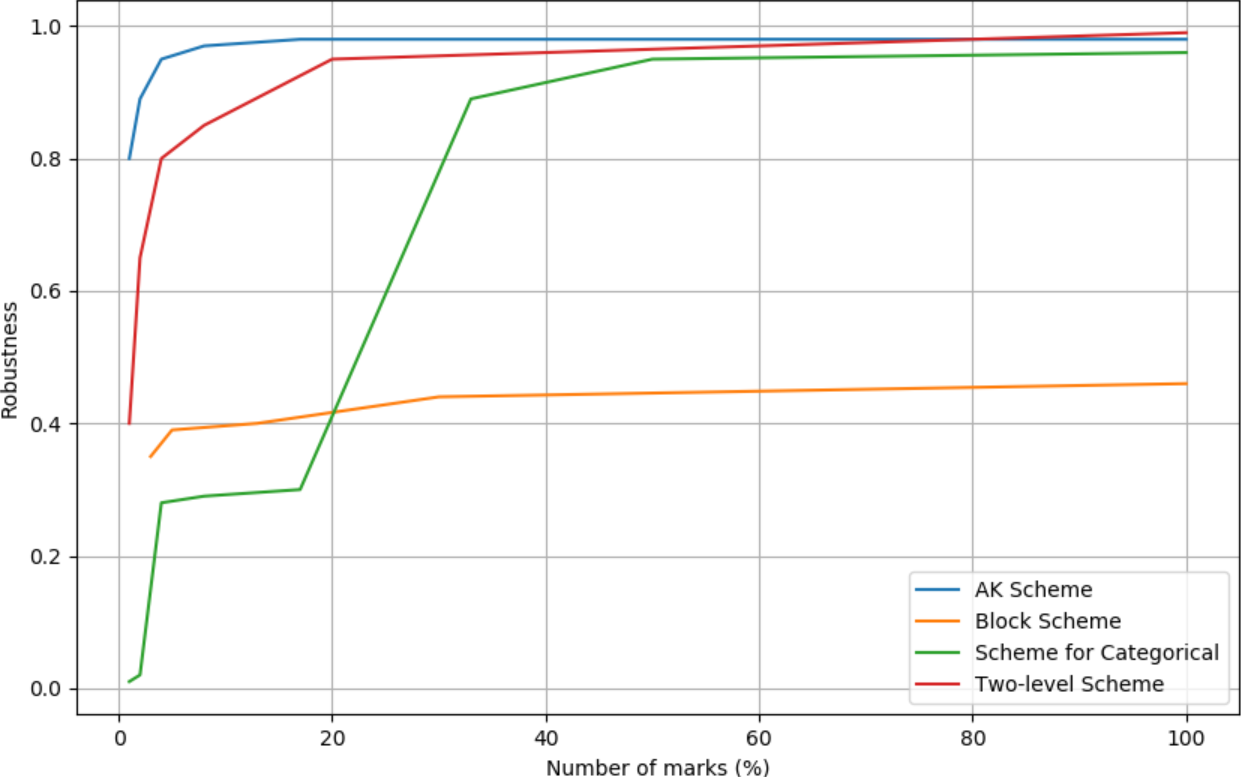
\includegraphics[width=\textwidth]{Figures/subset-screensh.PNG}
        \caption{Comparison of robustness against the subset attack}
        \label{fig:subset-attack}
    }\end{minipage}\hfill
    %bit-flipping
    \begin{minipage}{0.49\textwidth}
        \centering
        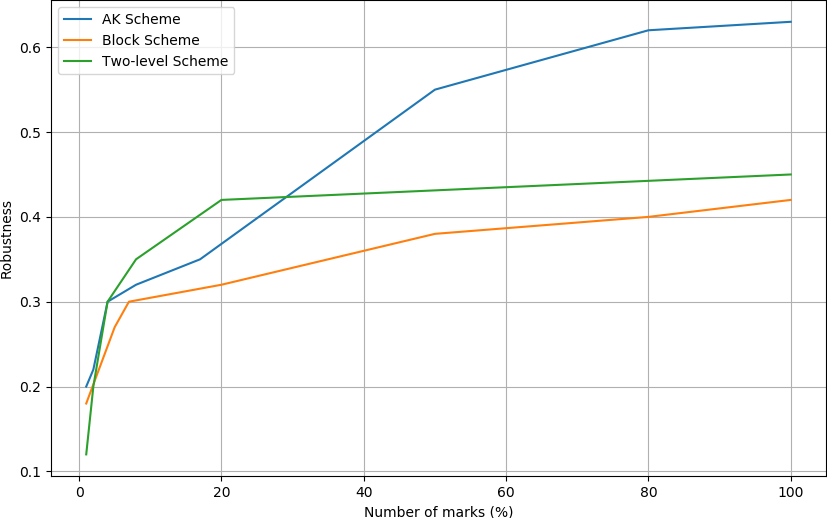
\includegraphics[width=\textwidth]{Figures/bit-flipping.PNG}
        \caption{Comparison of robustness against the bit-flipping attack}
        \label{fig:bit-flipping-attack}
    \end{minipage}
\end{figure}
Furthermore, we discussed the robustness against the attacks where the attacker modifies the dataset, e.g. subset attack and bit-flipping attack. A general conclusion is that more marks in the data mean better robustness. A somewhat smaller role plays the parameter $\xi$ that defines how many LSBs are available for fingerprinting such that is $\xi$ is bigger, the scheme is more robust. 
We compare the robustness of the discussed fingerprinting techniques against the subset attack in \Cref{fig:subset-attack} and the bit-flipping attack \Cref{fig:bit-flipping-attack}.
Robustness against the subset attack is measured as the largest percentage of tuples deleted where the scheme still detects the correct fingerprint with 100\% probability.
The AK Scheme shows the best robustness even for a smaller number of marks in the data. The Two-level Scheme and the scheme for categorical data are reaching a high robustness level for a larger number of marks in the data. The Block Scheme under-performs all the schemes.

Robustness of the bit-flipping attack is measured as the largest percentage of the LSBs that can be flipped while the scheme would still detect the correct fingerprint with probability 100\%.
AK Scheme again outperforms other schemes, except for the smaller number of marks where the Two-level Scheme is more robust. The Block Scheme is the least robust scheme against the bit-flipping attack. However, we can argue that all of the schemes are robust against the attack since they can all reach the level of robustness of $>0.4$.

We conclude that a good robustness level can be reached with a sufficient number of marks in the data. However, more marks in the data introduce more errors and they might significantly affect the utility of the data. In the next chapter, we will analyse how the utility is affected and if introducing the necessary number of marks to ensure the robustness is acceptable from the utility point of view.
